%%%%%%%%%%%%%%%%%%%%%%%%%%%%%%%%%%%%%%%%%%%%%%%%%%%%%%%%%%%%
%%% LIVECOMS ARTICLE TEMPLATE FOR BEST PRACTICES GUIDE
%%% ADAPTED FROM ELIFE ARTICLE TEMPLATE (8/10/2017)
%%%%%%%%%%%%%%%%%%%%%%%%%%%%%%%%%%%%%%%%%%%%%%%%%%%%%%%%%%%%
\documentclass[9pt]{livecoms}

%
% Command to make intext references not superscripted or bracketed
\makeatletter
\newcommand*{\citenumns}[2][]{%
  \begingroup
  \let\NAT@mbox=\mbox
  \let\@cite\NAT@citenum
  \let\NAT@space\NAT@spacechar
  \let\NAT@super@kern\relax
  \renewcommand\NAT@open{}%
  \renewcommand\NAT@close{}%
  \cite[#1]{#2}%
  \endgroup
}
\makeatother


\newcommand{\note}[1]{\textcolor{blue}{#1}}

\newcommand{\versionnumber}{0.1}  % you should update the minor version number in preprints and major version number of submissions.
\newcommand{\githubrepository}{\url{https://github.com/team-mayes/best_practice_pmf}}  %this should be the main github repository for this article

%%%%%%%%%%%%%%%%%%%%%%%%%%%%%%%%%%%%%%%%%%%%%%%%%%%%%%%%%%%%
%%% ARTICLE SETUP
%%%%%%%%%%%%%%%%%%%%%%%%%%%%%%%%%%%%%%%%%%%%%%%%%%%%%%%%%%%%
\title{Best Practices for Computing Free Energy Profiles and Potentials of Mean Force : v\versionnumber}

% Number is for affliation; add your name as you contribute; we can figure out order as the manuscript takes shape
\author[1]{Alan Grossfield}
\author[2]{Heather Mayes}
\affil[1]{University of Rochester}
\affil[2]{University of Michigan}
%\affil[3]{University 3}
%\affil[4]{Univ 4}
%\affil[5]{Affiliation 5}

%\corr{email1@example.com}{FMS}  % Correspondence emails.  FMS and FS are the appropriate authors initials.
%\corr{email2@example.com}{FS}

%\contrib[\authfn{1}]{These authors contributed equally to this work}
%\contrib[\authfn{2}]{These authors also contributed equally to this work}

%\presentadd[\authfn{3}]{Department, Institute, Country}
%\presentadd[\authfn{4}]{Department, Institute, Country}

\blurb{This LiveCoMS document is maintained online on GitHub at \githubrepository; to provide feedback, suggestions, or help improve it, please visit the GitHub repository and participate via the issue tracker.}


\begin{document}
\begin{frontmatter}
\maketitle

% TODO: revisit later; add in which methods we cover
\begin{abstract}
This document provides a starting point for calculating a potential of mean force and free energy profiles from molecular dynamics simulations. There are an increasing number of methods for this type of work. In the present guide, we introduce you to some of the popular current methods, as well as considerations to take into account no matter the method chosen. We point to further resources to gain a deeper understanding into the vibrant topic.
\end{abstract}
\end{frontmatter}

\section{Introduction}
% TODO: this is the outline from the meeting. Needs expansion.
% Up for task: Heather

The goal of this article is help researchers get started productively.
The theory is well laid out (add references) and many methods are available.
While some considerations are system dependent, we aim to provide overall guidelines.
In this document, we will introduce key terms and some common methods.

Note that we will not cover how to perform molecular simulations in this document. We refer readers to other best practices documents for introductory guides:
\begin{itemize}
\item MD basics \url{https://github.com/MobleyLab/basic_simulation_training}
\item MD setup, biomolecular setup \url{https://github.com/michellab/BioMolSetupPaper}
\item Statistical error and uncertainty analysis \url{https://github.com/dmzuckerman/Sampling-Uncertainty/}
\end{itemize}
You may want to review these first to check if you're comfortable with the material.

Additionally, we will not cover alchemical methods. 
% If they have a GitHub link, add it here)

Distinguish between methods that choose a coordinate a priori, and those that do not. We will mention those that do not (MSMs, TPS) but leave outside the scope.
In the scope will only be combinations of sampling and constructing PMFs from a priori chosen coordinates. Will discuss a first step of learning about the system and metastable states before choosing:
\begin{itemize}
\item US/Replica exchange
\item Metadynamics
\item Adaptive force biasing
\item Some on weighted ensemble
\end{itemize}

Restrict ourselves to a priori choices of RC. Mention that others exist
\begin{itemize}
\item approximate continuous function with discrete samples (most of the time)
\item Projection onto the state space
\item Histograms vs. laying down Gaussians
\item Histograms always underestimates barrier heights (not the worst problem)
\end{itemize}

MSM as an adaptive sampling method (will exclude this from our scope);
MSMs gives an RC but hard to relate to any theoretical condition, change temp, anything.
What are you going to do: RC for further sampling? If you want to generate low D representation MSMs are great; if want to discover an RC, TPS



There are many other enhanced sampling methods (multicanonical, Wang-Landau, Adaptive Umbrella Sampling, Tsallis statistics).  Can't cover them all. We can suggest reviews.

Discuss analysis of results with committor analysis.

\section{Key Terms}
% TODO: this is the outline from the meeting, plus some beginning of full sentences. Needs expansion.
% Up for task: Alan, Heather

Discuss both the definitions and actual use (not always strictly correct!)

\subsection{Potential of Mean Force}

%\section{Physical Meaning of free energy curves and potentials of mean force}
% !TEX root = ./best_pmf.tex

\label{s:phys_mean}

The configurational portion of the free energy of a system is computed via the partition function

\begin{equation}
    \label{e:partition}
    Z = \int d\vec{x} \exp{-U(\vec{x}/k_B T)}
\end{equation}

as

\begin{equation}
    A = -k_B T \ln Z
\end{equation}

The integrand of Eq. \ref{e:partition} can be thought of as the unnormalized
probability, since $\mathrm{prob} \propto \exp{-U(\vec{x}/k_B T)}$.  Thus, if we wish to compute the probability distribution along an arbitrary coordinate, we would write

\begin{equation}
    \label{e:prob}
    P(x) = \frac{1}{Z} \int d\vec{x'} J(x) \exp{-U(\vec{x', x}/k_B T)}
\end{equation}

\noindent where $\vec{x'}$ is all of the degrees of freedom in the system other
than $\vec{x'}$, and $J(x)$ is the Jacobian of $x$ (see below).  The free energy curve (also called a free energy profile) along $x$ can then be computed
as

\begin{equation}
    \label{e:free}
    A(x) = - k_B T \ln(P(x))
\end{equation}


The Jacobian in Eq. \ref{e:prob} accounts for the variation in the phase space
volume associated with the differential $d\vec{x}$ with $x$.  The depends on
precisely what $\vec{x}$ is. For example, if $\vec{x} = r $ is a distance in
3-dimensional space,

\begin{equation}
J(\vec{x}) = 4 \pi r^2
\end{equation}

\noindent Physically, this means that specifying $r$ traces out a sphere of
radius $r$, and $J(r)$ is the area of that sphere.  Similarly, if $\vec{x}=
\theta$, the tilt of a vector relative to the $z$-axis, then

\begin{equation}
J(\theta) = 2 \pi \cos(\theta)
\end{equation}

which would be the arc length of the circle traced out by a unit vector for a
specific value of $\theta$.

However, it is not always convenient to work in terms of probability, since this
contains information not only about the system, but also the chosen coordinate.
To separate the two, one can also work with the probability density

\begin{equation}
    \label{e:dens}
    \rho(x) = \frac{1}{Z} \int d\vec{x'} \exp{-U(\vec{x', x}/k_B T)}
\end{equation}

\noindent
The equivalent to Eq. \ref{e:free} defines the potential of mean force (PMF)

\begin{equation}
    \label{e:pmf}
    W(x) = - k_B T \ln(\rho(x))
\end{equation}

Comparing these two quantities, it is clear that, although the terms ``PMF'' and
``free energy curve'' are often used interchangeably, they are not by definition
the same unless $J(x)=1$.  Figure \ref{f:free} demonstrates this difference for the case of a pair of ideal gase particles.

\begin{figure}
\centering
    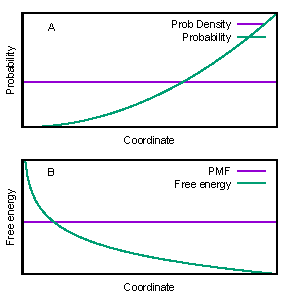
\includegraphics[width=5.8cm]{figures/ideal_gas/free}
    \caption{\label{f:free}
    Free energy curves vs. potentials of mean force.  Panel A shows the probability density and probability curves for the case where the chosen variable is the distance between 2 ideal gas particles.  The probability density is constant, while the probability increases with distance.  Panel B shows the equivalent free energy quantities, as computed by Eqs. \ref{e:free} and \ref{e:pmf}.
    }
\end{figure}

% TODO: discuss when you want PMF and when you want free energy
% TODO: discuss which methods produce what
 % Alan Grossfield

PMF (analogous to probability density)  vs free energy surface (analogous to probability); Only ABF gives a PMF, umbrella sampling and metadynamics give free energy curves.

PMF is a free energy as a function of almost, but not all the coordinates:
\begin{itemize}
\item PMF(x0,x1. . . ) = -kb T log x  x0,x1 exp(- beta U(x)) dx (all but x0, x1)
\item Only defined up to a constant.
\item write equation to show distinction between PMF and free energy
\item Jacobian correction
\begin{itemize}
\item Common jacobians -- distance ($ J= 4 \pi r^2$), angles (J = 1)
\item Other common rxn coords J is unknown (native contacts, RMSD)
\item Make a figure showing free energy and PMF for a couple of simple systems (2 ideal gas particles, 2 LJ particles?)
\end{itemize}
\end{itemize}

PMF is a fundamentally a continuous function (unless the rxn coord is intrinsically discrete), but we have to approximate the continuous function when we estimate it. Two approaches to approximate:
\begin{itemize}
\item Expectations of histograms or other indicator functions
$\Delta A(xi) = \sum_{k=1}^K \sum_{n=1}^N \sum W_i(x_n) I_k(x_n)$, where $I_k$ is some local indicator function, like a top hat function centered at $x_n$, or a gaussian centered at $x_n$.
\item Some sort of fit from the data to a continuous function with different parameters, for example by a least squares fit or Kullbeck-Liebler divergence. (refs)  Useful if you're using the curves as input to simpler calculations
\end{itemize}

\subsection{What is the reaction coordinate/OP/CV?}
%From the theory of phase transitions:

\begin{itemize}

  \item \textbf{Potential of mean force (PMF)} is formally the ``potential'' derived by integrating the mean force along a path or coordinate \cite{Kirkwood-1935}, analogous to the probability density along that coordinate.  Often used interchangeably with \textbf{Free energy curve}, but strictly the PMF does not contain entropic contributions from the Jacobian of the chosen coordinate.

  \item \textbf{Free energy curve} is the free energy as a function of a
  particular coordinate or coordinates.  It is directly related to the
  probability distribution along that coordinate, and implicitly includes the
  entropic contributions from the Jacobian.


  \item \textbf{Collective variable (CV):} any variable composed of displacements of
  multiple particle coordinates.  It could be as simple as the distance between
  two particles, or complex like the fraction of native contacts present in a
  protein folding simulation.

  \item \textbf{Order parameter:}  a collective variable that distinguishes between two or more stable states

  \item \textbf{Reaction coordinate (RC):} the pathway followed by a chemical reaction or conformational change.  Often used interchangeably with collective variable.

\end{itemize}

\section{Considerations before you start computing}
% TODO: check the outline below and delete is covered in the text written so far
% Up for task: Allan

%Is the question well-posed? Is the project doable?
%   - Sturgeon’s law as an organizing principle (“Ninety percent of everything is crud”) -- what can we do to drop the percentage?
%   -Recommend starting with conventional MD (possibly with T Rep Ex) to understand the system
%   - What is the choice for (x0,x1, . . . ) that you don’t integrate over?
%      - Careful choice needed, poor choice uninformative or misleading
%      - All choices are true, only some are useful or informative.
%         - if you try to interpret mechanism, you're asserting that all other degrees of freedom are fast (and thus in equilibrium) with respect to the chosen ones.
%      - What are relevant degree or degrees of freedom?
%   - What kinds of barriers are expected along the reaction coordinate?
%   - Lengthscale of features on reaction coordinate   
%   - Timescales for relaxation of orthogonal degrees of freedom? How long do individual trajectories need to be?  
%   - Can we implement the reaction coordinate efficiently as a bias?
%      - Most packages implement some simple restraints
%      - Plugins: COLVARS, PLUMED
%   - How many dimensions?
%      - Usually, people only do 1 or 2 dimensions.
%      - More dimensions makes it more complicated, both to compute, and more importantly to understand what the heck is going on.  Most of the recommendations will be for 1 and 2 dimensions, with a separate section for ndim > 2.


\subsection{Checklist for designing a free energy profile calculation}
% !TEX root = ./paper.tex

\section{Checklist for designing a free energy profile calculation}
\label{s:precheck}

% Note from AMG: I'm putting a lot of text in the checklist, but
% we might want to break that text out into the body of the document.

The first key to a successful outcome is appropriate experimental design.  That is, you first need to ensure that the calculation is plausibly doable given the resources available, and that the question is is well-posed.  The following is a list of items that must be considered before beginning such a calculation.  Answering these questions will help you decide which techniques

\begin{itemize}

    \item \textbf{What collective variable or variables will be used as reaction
    coordinate?}  The statistical physics of free energy curves gives us
    considerable leeway in choosing our reaction coordinates --- in principle,
    any variable could be used, and if the calculation is performed correctly
    the resulting free energy curve will be ``true''.  However, as a practical
    matter, interpreting the curve will be challenging (or even deceptive)
    unless the reaction coordinate is a good approximation to the true
    mechanism.

    \item \textbf{What are the other relevant motions in the system? On what
    timescale do they take place?}  The derivation of a free energy curve
    involves computing a thermodynamic average over all degrees of freedom in
    the system other than the chosen path.  In practical terms, this means that
    any slow degrees of freedom in your system that aren't explicitly biased or
    tracked must be sampled for the results to converge statistically.  This is
    particularly problematic if there are multiple slowly exchanging states not
    explicitly spanned by the chosen collective variable.

    \item \textbf{What is the expected ``lengthscale'' of features on the
    reaction coordinate?}  Over what range will the collective variables be
    tracked? How finely do we need to determine the free energy curve to be able
    to answer the scientific question?

    \item \textbf{Can the reaction coordinate be used to calculate a biasing
    energy or force? }  Many techniques, such as metadynamics and umbrella
    sampling, make direct use the chosen collective variables by adding
    additional biasing forces to the simulation.  Thus, when using one of these
    techniques, one is restricted to collective variables that can easily be
    computed on the fly in the simulation, preferably without greatly reducing
    computational performance.

    \item \textbf{How many collective variables do you plan to bias?} There's a
    challenging tradeoff here: If there are slow degrees of freedom you don't
    bias, you may effectively just be doing brute force sampling.  On the other
    hand, the number of trajectories typically increases exponentially with the
    number of collective variables biased.  As a result, it is very rare that you see more than 1 or 2 dimensional enhanced sampling.

    \item \textbf{Are the barriers expected to enthalpic, entropic, or both? Are
    there major entropic differences between states?}  Different enhanced
    sampling methods do better with different kinds of biases.  For example,
    conventional replica exchange is great for purely enthalpic barriers
    (raising the temperature exponentially increases the rate of barrier
    crossing) but is less helpful with entropic ones (the only gain at high
    temperature is an increase in the ``diffusion'' constant).  Thinking about
    the kinds of barriers involved should inform your choice of enhanced
    sampling technique.

\end{itemize}
 % Alan Grossfield

\section{Selecting collective variables for sampling}

[Andy F]

\begin{itemize}
\item Intuition / experience based selection of CVs
\item ``Perils of projection'' -- hidden barrier problem, artificial collapse of kinetically distinct states
\item Number of CVs and curse of dimensionality -- exponential increase in sampling cost with number of CVs
\item Post-hoc projection into CVs other than those in which sampling was conducted \cite{ferguson2017bayeswham}
\item Requirement for explicit (MC) and differentiable (MD) expressions for CVs in terms of atomic coordinates
\item Systematic techniques for CV discovery (PCA, Isomap, LLE, dMaps, ANNs)
\end{itemize}

\section{Sampling techniques}
% TODO: this is the outline from the meeting. Needs expansion.
% Up for task: ?

Mention what they do.
\begin{itemize}
\item Restrict ourselves to conventional/T Rep EX, US / HREx , Metadynamics, and adaptive force biasing; add strengths and weaknesses of each method (dynamic range to be surmounted)
\item Conventional MD / T Rep Ex (conventional histogram; MSM to analyze)
\item Direct counting/MSM: Usually bad, because only samples the minima, not the barriers.  Will fail even in the absence of barriers -- just need a significant (> 5 kT, maybe) range of free energies
\item Umbrella sampling / Ham Rep Ex (need weighted)
\item Design simulation so it can be tested (Prefer running each window multiple times, construct as independently as possible, best way to get error bars)
\item Tests for convergence and self-consistency. For Ham Rep Ex\cite{Neale2014}
\item Uncertainty quantification and error estimation -- bootstrap resampling, Gibbs / MC sampling of Bayes posterior
\end{itemize}

\section{Computing the free energy/PMF from US/Ham Rep Ex}
% TODO: this is the outline from the meeting. Needs expansion.
% Up for task: Alan for WHAM; others for other sections?

%   - WHAM
%      - Several implementations: mine (http://membrane.urmc.rochester.edu/content/wham), g_wham in gromacs, built in to CHARMM
%      - Special case for extreme range of free energies: https://github.com/dejunlin/gwham
%      - Minimal tests you need to do
%         - Check that histograms overlap
%         - Check that bin size is small enough that it’s not altering the answer
%         - Tolerance must be small enough that the PMF isn’t changing
%         - Make sure units match
%            - Mention Amber issue with angle restraints as example
%         - Make sure factor of 1/2 matches
%         - This is the terminology from Grossfield's WHAM, look at g_wham, etc and check how they talk about it
%      - Computing other properties using umbrella-sampled data
%         - In principle, WHAM can do it, but probably not the best choice because it's harder to control histogramming artifacts. Recommend
%         MBAR
%   - MBAR (https://github.com/choderalab/pymbar), also an implementation in Toni Mey's github repo, add link
%      - @mrshirts: insert something smart here. :)
%   - TRAM would also be a method to compute a pmf (https://github.com/markovmodel/thermotools/tree/devel/ext) (combine weighted and unweighted)
%      - Ask Toni Mey to insert something smart here

\subsection{Computing free energy profiles using WHAM}
% Alan Grossfield
% !TEX root = ./paper.tex

\subsection{Computing free energy profiles using WHAM}

The most common way to extract a free energy profile from umbrella sampling data
is the weighted histogram analysis method, or WHAM \cite{Swendsen-1995, Roux-1995, Swendsen-1992}.
For the most common case, where all
trajectories were run at the same temperature and the bias is solely a function
of the collective variable, the two key WHAM equations are

EQUATIONS HERE, USING MY OLD NOTATION

where DEFINE TERMS HERE. Each trajectory is histogrammed along the chosen
collective variable, and thus produced a biased estimate of the probability
distribution. If there were only one trajectory, the WHAM equations would reduce
to simple thermodynamic reweighting, but with multiple estimates from the
various trajectories one must compute some kind of weighted average.  The  $F_i$
values serve precisely this purpose; the WHAM derivation shows that iteratively
solving these equations minimizes the variance in the resulting probability
distribution.

There are a number of WHAM implementations available.  Probably the most commonly used one is due to Grossfield \cite{WHAM}, but there are also version included as part of gromacs \cite{Lindahl-2013} and CHARMM \cite{CHARMM2009}.

Although WHAM is a robust method, there are a number of checks one should apply
to any calculation performed with it (this is in addition to the design-level
tests discussed in Section \ref{s:precheck}).

\begin{itemize}

    \item \textbf{Check that your units are consistent}.  Many WHAM codes are
    agnostic to the choice of collective variable, but do require that the units
    be consistent.  Specifically, most implementations assume the restraints are
    harmonic in the reaction coordinate, and thus expect that if the time series
    are given in units of $X$ (e.g. {\AA} or nm for a distance), the restraint's
    spring constant is given in units of $\mathrm{energy}/X^2$, and will output
    the free energy curve in units of $\mathrm{energy}$.  There are known issues
    with some simulation packages. Most notably, when restraining angles or
    torsions in Amber, the location of the restraint minimum is specified in
    degrees (as is the output), but the restraint is specified in radians.  This
    mismatch is dramatic enough to cause the WHAM calculation to fail
    immediately, generally producing all ``NaN'' values for the free energy
    curve.

    \item \textbf{Check the functional form of the restraint}.  Although most
    packages use harmonic restraints, some include a prefactor of 0.5, while
    others do not.  To produce correct results, you may need to given a
    different value to the WHAM code than you did to the simulation package.
    For example, NAMD and Amber restraints restraints do not use the prefactor,
    while Grossfield's WHAM does, so if you ran a NAMD simulation with a spring
    constant of 10 kcal/{\AA}$^2$, you would put 20 as the spring constant in
    the WHAM metadata file.

    \item \textbf{Verify the histograms overlap}.  If there are ``bare'' patches
    (or even just poorly sampled regions), the free energy profile will not be
    reliable.  This test should be performed \emph{before} running WHAM; WHAM
    works best when the total number of samples is roughly constant across the
    whole range of the collective variable.

    \item \textbf{Make sure the iteration is fully converged}.  The WHAM
    equations are generally solved by iteration to self-consistency, so it is
    crucial to ensure that the iteration has proceeded far enough that the
    answer is not changing.  You should check the manual for your chosen WHAM
    implementation for a suggested value, but also should (if possible) plot the
    intermediate free energy curves to verify they've stopped changing.  If the
    range of values on your free energy curve is especially large (hundreds of
    $k_B T$), there may be significant issues with numerical precision
    preventing the curves from converging.  In this case, you can use a
    special-purpose WHAM implementation intended to handle this case, available
    from \url{https://github.com/dejunlin/gwham}.

    \item \textbf{Check that the chosen bin width isn't altering the answer}.
    Finite-width histogram bins intrinsically smooth the free energy profile by
    breaking it into regions.  This effect can be minimized (and often
    effectively eliminated) by reducing the bin size, at the cost of reducing
    the number of samples in each bin, which makes the curve noisier.  To verify
    that the bin width isn't a problem, one should always re-run WHAM several
    times with different bin width to verify that the resulting curve does not
    vary systematically.  The key is that the bins must be narrower than the
    relevant ``features'' of the free energy curve; bins comparable to or
    broader than these features with obscure them or even smooth them away.

\end{itemize}

It is also crucial to assess whether other relevant orthogonal degrees of
freedom (variables other than the one used as a collective variable) are
well-sampled.  This is a complex general problem, so we can't give you a simple
test.  Rather, you have to honestly look at your system, and verify that
overlapping trajectories are genuinely similar (and not just similar according
to the collective variable).  The only automated procedure for looking for
problems that we are aware of is due to Neale et al \cite{Pomes-2014}, and only
applies to the case where the umbrella sampling was performed using Hamiltonian
replica exchange; in essence, the method looks for regions of the collective
variable where there is hysteresis in the migration of the trajectories up and
down the variable range as evidence for slow orthogonal relaxation.
 

%- Metadynamics (well-tempered metadynamics)
%   - why choose which variant of metadynamics
%   - risks of choosing too fact an annealing time in well-tempered
%   - Use estimator from bias vs. run for a while, then fix the bias and sampling on that then reweight (in which case you're probably better off just using original metadynamics)
%   - One of the people we've discussed inviting should really write this
%
%- Weighted ensemble; good for complex/computationally expensive reaction coordinates
%   - explain the principle, link to original Huber and Kim 1996 and Chong and Zuckerman 2017
%   - advantage is that you don't need to put the bias into the dynamics
%      - great for complex or expensive reaction coordinates
%      - gives correct kinetics for free in additional to free energy curve
%      - WESTPA as reference implementation
%- Adaptive biasing force--samples and computes PMF
%   - Extended ABF
%   - Do we need an expert on this? Jerome Henin maybe?

\section{Projection of computed PMF into alternative CVs}

[Andy F] Reweighting of PMF into arbitrary CVs other than those in which sampling was conducted \cite{ferguson2017bayeswham}

\section{Analysis common to all methods}
% TODO: this is the outline from the meeting.
% Up for task: ?

%%- Signatures of what has gone wrong within post-processing/ troubleshooting guide
%%   - Units (open MM is good, Amber has inconsistent units in angle restraints)
%%   - Stupid factor of 2 prefactors are inconsistent across codes
%%   - Error
%%   - Show some plots of what “bad” data will look like
%%      - I have some examples on butane I can dig up
%%- Signatures of what has gone wrong in the simulation itself
%%   - Hysteresis
%%   - Slow relaxation -- trim off the front of individual windows, look for systematic change in the resulting curve, cite Neale and Pomes
%%   - Look for structural similarity in neighboring bins
%%   - Look for hidden orthogonal barriers in HamRepex by failed replica percolation (Neale and Pomes)
%%- Committor analysis to verify you've found transition state
%%- Computing error bars on PMFs / free energy curves
%%   - Bootstrapping, etc: needs correlation as input, not particularly reliable.  
%%      - Not necessarily the correlation time of the rxn coord
%%      - Example: ion through ion channel, z-fluc of ion is faster than protein fluctuations
%%- Do multiple independent runs
%%- PMF only defined up to constant, how do you align curves to get error bars
%%   - Several possible solutions (matrix of differences, bin-to-bin differences) credit Chodera, Louis Smith came up with bin-to-bin diffs, not published
%
% Include “Good ideas that didn’t work”? -- examples of problems in PMF calculations
%Suggestion by Dan Zuckerman
%E.g. “I chose the wrong reaction coordinate and it ruined my life”
%


\clearpage

\renewcommand\bibnumfmt[1]{#1.}
\bibliography{best_pmf}
\bibliographystyle{vancouver-livecoms}

\end{document}
